% Options for packages loaded elsewhere
\PassOptionsToPackage{unicode}{hyperref}
\PassOptionsToPackage{hyphens}{url}
\PassOptionsToPackage{dvipsnames,svgnames,x11names}{xcolor}
%
\documentclass[
  super,
  preprint,
  3p]{elsarticle}

\usepackage{amsmath,amssymb}
\usepackage{iftex}
\ifPDFTeX
  \usepackage[T1]{fontenc}
  \usepackage[utf8]{inputenc}
  \usepackage{textcomp} % provide euro and other symbols
\else % if luatex or xetex
  \usepackage{unicode-math}
  \defaultfontfeatures{Scale=MatchLowercase}
  \defaultfontfeatures[\rmfamily]{Ligatures=TeX,Scale=1}
\fi
\usepackage{lmodern}
\ifPDFTeX\else  
    % xetex/luatex font selection
\fi
% Use upquote if available, for straight quotes in verbatim environments
\IfFileExists{upquote.sty}{\usepackage{upquote}}{}
\IfFileExists{microtype.sty}{% use microtype if available
  \usepackage[]{microtype}
  \UseMicrotypeSet[protrusion]{basicmath} % disable protrusion for tt fonts
}{}
\makeatletter
\@ifundefined{KOMAClassName}{% if non-KOMA class
  \IfFileExists{parskip.sty}{%
    \usepackage{parskip}
  }{% else
    \setlength{\parindent}{0pt}
    \setlength{\parskip}{6pt plus 2pt minus 1pt}}
}{% if KOMA class
  \KOMAoptions{parskip=half}}
\makeatother
\usepackage{xcolor}
\setlength{\emergencystretch}{3em} % prevent overfull lines
\setcounter{secnumdepth}{5}
% Make \paragraph and \subparagraph free-standing
\ifx\paragraph\undefined\else
  \let\oldparagraph\paragraph
  \renewcommand{\paragraph}[1]{\oldparagraph{#1}\mbox{}}
\fi
\ifx\subparagraph\undefined\else
  \let\oldsubparagraph\subparagraph
  \renewcommand{\subparagraph}[1]{\oldsubparagraph{#1}\mbox{}}
\fi


\providecommand{\tightlist}{%
  \setlength{\itemsep}{0pt}\setlength{\parskip}{0pt}}\usepackage{longtable,booktabs,array}
\usepackage{calc} % for calculating minipage widths
% Correct order of tables after \paragraph or \subparagraph
\usepackage{etoolbox}
\makeatletter
\patchcmd\longtable{\par}{\if@noskipsec\mbox{}\fi\par}{}{}
\makeatother
% Allow footnotes in longtable head/foot
\IfFileExists{footnotehyper.sty}{\usepackage{footnotehyper}}{\usepackage{footnote}}
\makesavenoteenv{longtable}
\usepackage{graphicx}
\makeatletter
\def\maxwidth{\ifdim\Gin@nat@width>\linewidth\linewidth\else\Gin@nat@width\fi}
\def\maxheight{\ifdim\Gin@nat@height>\textheight\textheight\else\Gin@nat@height\fi}
\makeatother
% Scale images if necessary, so that they will not overflow the page
% margins by default, and it is still possible to overwrite the defaults
% using explicit options in \includegraphics[width, height, ...]{}
\setkeys{Gin}{width=\maxwidth,height=\maxheight,keepaspectratio}
% Set default figure placement to htbp
\makeatletter
\def\fps@figure{htbp}
\makeatother

\usepackage{booktabs}
\usepackage{caption}
\usepackage{longtable}
\usepackage{colortbl}
\usepackage{lineno}\linenumbers
\makeatletter
\makeatother
\makeatletter
\makeatother
\makeatletter
\@ifpackageloaded{caption}{}{\usepackage{caption}}
\AtBeginDocument{%
\ifdefined\contentsname
  \renewcommand*\contentsname{Table of contents}
\else
  \newcommand\contentsname{Table of contents}
\fi
\ifdefined\listfigurename
  \renewcommand*\listfigurename{List of Figures}
\else
  \newcommand\listfigurename{List of Figures}
\fi
\ifdefined\listtablename
  \renewcommand*\listtablename{List of Tables}
\else
  \newcommand\listtablename{List of Tables}
\fi
\ifdefined\figurename
  \renewcommand*\figurename{Figure}
\else
  \newcommand\figurename{Figure}
\fi
\ifdefined\tablename
  \renewcommand*\tablename{Table}
\else
  \newcommand\tablename{Table}
\fi
}
\@ifpackageloaded{float}{}{\usepackage{float}}
\floatstyle{ruled}
\@ifundefined{c@chapter}{\newfloat{codelisting}{h}{lop}}{\newfloat{codelisting}{h}{lop}[chapter]}
\floatname{codelisting}{Listing}
\newcommand*\listoflistings{\listof{codelisting}{List of Listings}}
\makeatother
\makeatletter
\@ifpackageloaded{caption}{}{\usepackage{caption}}
\@ifpackageloaded{subcaption}{}{\usepackage{subcaption}}
\makeatother
\makeatletter
\@ifpackageloaded{tcolorbox}{}{\usepackage[skins,breakable]{tcolorbox}}
\makeatother
\makeatletter
\@ifundefined{shadecolor}{\definecolor{shadecolor}{rgb}{.97, .97, .97}}
\makeatother
\makeatletter
\makeatother
\makeatletter
\makeatother
\journal{npj Digital Medicine}
\ifLuaTeX
  \usepackage{selnolig}  % disable illegal ligatures
\fi
\usepackage[]{natbib}
\bibliographystyle{elsarticle-num}
\IfFileExists{bookmark.sty}{\usepackage{bookmark}}{\usepackage{hyperref}}
\IfFileExists{xurl.sty}{\usepackage{xurl}}{} % add URL line breaks if available
\urlstyle{same} % disable monospaced font for URLs
\hypersetup{
  pdftitle={Improving Sleep Quality Estimation: A Comparative Study of Machine Learning and Deep Learning Techniques Utilizing Free-Living Accelerometer Data from Thigh-Worn Devices and EEG-Based Sleep Tracking},
  pdfauthor={Esben Høegholm Lykke; Jan Christian Brønd},
  pdfkeywords={Sleep, Accelerometry, EEG, Machine learning, Sleep
quality},
  colorlinks=true,
  linkcolor={blue},
  filecolor={Maroon},
  citecolor={Blue},
  urlcolor={Blue},
  pdfcreator={LaTeX via pandoc}}

\setlength{\parindent}{6pt}
\begin{document}

\begin{frontmatter}
\title{Improving Sleep Quality Estimation: A Comparative Study of
Machine Learning and Deep Learning Techniques Utilizing Free-Living
Accelerometer Data from Thigh-Worn Devices and EEG-Based Sleep Tracking}
\author[1]{Esben Høegholm Lykke%
\corref{cor1}%
}
 \ead{eskovgaard@health.sdu.dk} 
\author[1]{Jan Christian Brønd%
%
}
 \ead{jbrond@health.sdu.dk} 

\affiliation[1]{organization={University of Southern Denmark, Department
of Sports Science and Clinical Biomechanics},addressline={Campusvej
55},city={Odense},postcode={5230},postcodesep={}}

\cortext[cor1]{Corresponding author}


        
\begin{abstract}
LÆS IKKE! Det er volapyk på latin. Lorem ipsum dolor sit amet,
consectetur adipiscing elit. Suspendisse vitae dictum eros, ullamcorper
elementum orci. Sed laoreet nulla neque, pulvinar fermentum mi iaculis
at. Nulla ultricies nibh sit amet vestibulum rutrum. Nam pharetra nisl
sed ipsum maximus suscipit. Duis metus nunc, ullamcorper eu mi rutrum,
tempus ultricies ante. Nunc vitae lectus nisi. Aliquam efficitur ut eros
ut pellentesque. Aenean blandit, nisl nec efficitur interdum, nisi ipsum
fermentum dolor, at tempus sem turpis in lacus. Curabitur sollicitudin
lectus sit amet velit pellentesque laoreet. Ut posuere diam lobortis
nisi eleifend tincidunt. Ut at euismod sem, sed dignissim ligula.
Aliquam lacinia massa libero, id eleifend velit pulvinar ac. Fusce
volutpat elit eu nulla viverra, nec tempus orci pellentesque.
\end{abstract}





\begin{keyword}
    Sleep \sep Accelerometry \sep EEG \sep Machine learning \sep 
    Sleep quality
\end{keyword}
\end{frontmatter}
    \ifdefined\Shaded\renewenvironment{Shaded}{\begin{tcolorbox}[breakable, borderline west={3pt}{0pt}{shadecolor}, boxrule=0pt, frame hidden, enhanced, sharp corners, interior hidden]}{\end{tcolorbox}}\fi

\hypertarget{introduction}{%
\section{Introduction}\label{introduction}}

A vast body of research highlights the critical role of sleep in
maintaining both mental and physical
health\citep{ma2017, meyer2022, kpavlova2019, difrancesco2019}.
Consequently, accurate sleep assessment methods are crucial for tracking
sleep patterns and improving our understanding of the sleep-health
relationship. Furthermore, the ease of use and high acceptability of
these methods are essential to facilitate large-scale, longitudinal
studies.

While laboratory-based polysomnography (PSG) is typically considered the
gold standard for objective sleep measurement, its practicality in
large-scale epidemiological studies is hindered due to high costs, the
necessity for professional administration, and it is also subject to
potential rater bias\citep{vandewater2011, lee2022}. As an alternative,
diaries are commonly employed as cost-effective and low-tech methods for
sleep assessment in population research. However, reliance on
diary-based methods may lead to recall bias and other
limitations\citep{moore2015}. A more feasible approach in large-scale
epidemiological studies is to use device-based measurement methods that
can estimate sleep duration. This approach offers the advantage of being
less burdensome for participants and eliminates potential biases
associated with recall.

Body-worn accelerometers have emerged as an effective and affordable
alternative for objectively assessing sleep patterns at home over
extended periods. These devices gather continuous, high-resolution data
for several weeks without the need for recharging, thus reducing
participant burden. Initial applications of accelerometry for sleep and
wake stage classification were based on wrist movements, starting with
an algorithm developed in 1982 and validated with PSG
\citep{webster1982}. This model was later refined in 1992
\citep{cole1992}, giving rise to the widely used Cole-Kripke model. As
the field advanced, an array of techniques, including heuristic
algorithms, machine learning models, regression, and deep learning, were
employed to analyze wrist-worn accelerometer
data\citep{palotti2019, cole1992, sazonov2004, sadeh1994, hees2015, sundararajan2021}.

While wrist and hip-worn devices have benefited from extensive
methodological development, thigh-worn accelerometers have not seen the
same level of advancement. Existing studies mainly focus on
distinguishing sleep from wakefulness, with emphasis on defining `waking
time' and `bedtime'
\citep{carlson2021, inan-eroglu2021, vanderberg2016, winkler2016}.
Recent strides in estimating sleep duration using these devices have
been made, including the introduction of a promising algorithm and its
comparison against PSG\citep{johansson_development_2023}. Despite these
advancements, the application of machine learning techniques in this
area is still relatively unexplored. Considering the potential of
thigh-worn accelerometers for accurate physical behavior
assessment\citep{skotte_detection_2014, arvidsson2019}, there is a
significant research gap. Therefore, future studies need to develop
techniques similar to those used for wrist and hip-worn accelerometers,
with the ultimate goal of establishing a more holistic, accurate, and
user-friendly method of sleep and physical activity tracking.

The Zmachine®️ Insight+ (ZM) emerges as a valuable tool within this
landscape. Favorably validated against PSG\citep{kaplan2014, wang2015},
the ZM provides comparable data without the high costs or the need for
professional monitoring typically associated with PSG. Crucially, the ZM
facilitates multi-night analysis in free-living conditions due to its
ease of use\citep{pedersen2021}, capturing the natural variations in
sleep patterns. This makes it advantageous over single-night PSG,
particularly as a gold standard data source in machine learning tasks,
as it provides multiple nights of measurements without inter-rater bias.
Despite these benefits, the ZM, like PSG, still poses a significant
participant burden and cost, reinforcing the need for more accessible
alternatives like accelerometers.

Our primary objective in this study was to evaluate a range of machine
learning and deep learning models, utilizing the raw data collected from
a tri-axial thigh-worn accelerometer to estimate in-bed and sleep time.
To ensure the reliability and effectiveness of our models, we compared
their outputs with an EEG-based sleep tracking device, which we
considered the gold standard for measuring sleep. Furthermore, our
secondary goal was to assess the developed models' performance in
evaluating important sleep quality parameters, including sleep period
time (SPT), total sleep time (TST), sleep efficiency (SE), latency until
persistent sleep (LPS), and wake after sleep onset (WASO).

\hypertarget{methods}{%
\section{Methods}\label{methods}}

\hypertarget{dataset-and-participants}{%
\subsection{Dataset and participants}\label{dataset-and-participants}}

The current study leverages data from the SCREENS
project\citep{rasmussen2020}, a study conducted from October 2018 to
March 2019 in Middelfart, Southern Denmark, that evaluated the impact of
screen media usage on Danish families. For our analysis, we focused on
data from child participants aged between 6 and 10 years within the
SCREENS cohort. Our primary sources of data were accelerometer readings
from Axivity AX3 devices attached to the children's thighs, and
electroencephalography (EEG) data derived from the ZM device. The
Axivity AX3, an unobtrusive 3-axis accelerometer, was positioned midway
between the hip and knee on the right anterior thigh, recording
participant movement data.

Sleep state information was extracted using the ZM, a product of General
Sleep Corporation. The ZM, which utilizes advanced EEG hardware and
signal processing algorithms, employs three self-adhesive, disposable
sensors placed outside the hairline for reliable EEG signal acquisition.
The ZM uses two proprietary algorithms: Z-ALG and Z-PLUS. The Z-ALG is
utilized for accurate sleep detection, showcasing its suitability for
in-home monitoring\citep{kaplan2014}, while the Z-PLUS effectively
differentiates sleep stages, as evidenced by its alignment with expert
evaluations using PSG data\citep{wang2015}. In the current study, we
treated all sleep stages as a single category effectively deducing the
output of the ZM to ``awake'' and ``asleep'' as the ability to
distinguish sleep stages are not a necessity to derive sleep quality
parameters of interest and to simplify the learning process of the
models.

Figure~\ref{fig-flow} illustrates the selection criteria applied to the
children's recordings from the SCREENS study. We included only ZM
recordings that were accompanied by complete accelerometer data and
lasted between 7 and 14 hours. Any night when the ZM reported sensor
issues was excluded. The children whose recordings were considered had
an average age of 9.4 years, with a standard deviation of 2.1. In their
raw form, the ZM predictions encompassed 696,779 epochs, each 30 seconds
long. Notably, approximately 84\% of the total ZM recording duration was
classified as sleep, resulting in an imbalance of the dataset.

\begin{figure}[b]

{\centering 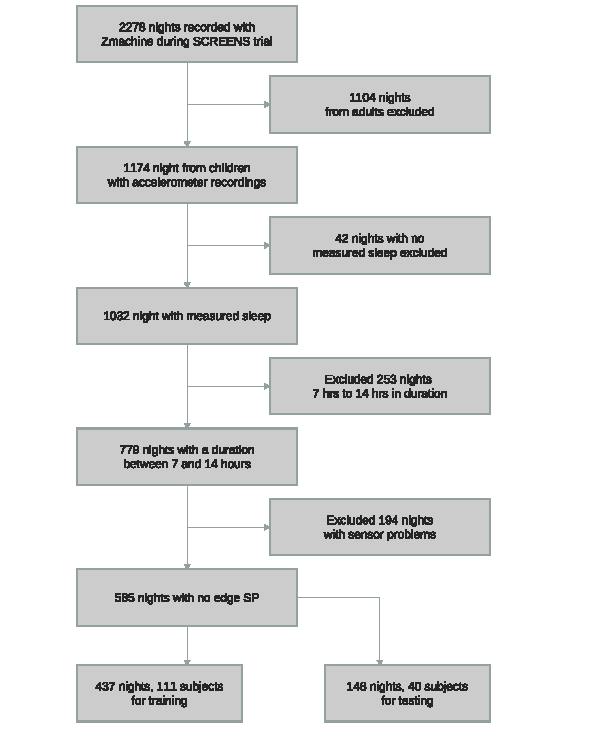
\includegraphics{visuals/flowchart_of_elligible_nights.pdf}

}

\caption{\label{fig-flow}Flowchart of eligible ZM recording nights
included in the study}

\end{figure}

Finally, we affirm that the SCREENS study received approval from the
Regional Scientific Committee of Southern Denmark, and all data handling
processes complied with the General Data Protection Regulation (GDPR),
ensuring the ethical and secure management of participant information.

\hypertarget{data-preprocessing-and-feature-extraction}{%
\subsection{Data Preprocessing and Feature
Extraction}\label{data-preprocessing-and-feature-extraction}}

In this study, data processing of the raw accelerometer data began with
a low-pass filtration step using a 4th order Butterworth filter with a 5
Hz cut-off frequency to eliminate high-frequency noise. Following
filtration, data were partitioned into overlapping 2-second intervals,
each successive interval sharing a 50\% overlap with the previous one
similar to methods described by Skotte et
al.\citep{skotte_detection_2014}. Any non-wear data was remove using
previously described methods\citep{skovgaard2023} and data was resampled
to 30-second epochs so every sample classified by the algorithms
corresponds to a 30-second epoch scored during the ZM recordings.
Subsequently, we performed a feature extraction process that yielded a
set of 88 features, providing a robust characterization of the data.
Extracted from accelerometer and temperature signals, these features
include temporal elements that use both lag and lead values, capturing
dynamic data trends by incorporating measurements from preceding and
upcoming intervals. Furthermore, inspired by Walch et
al.\citep{walch2019}, we incorporated sensor-independent features to
encapsulate circadian rhythms. These features offer unique insights not
directly discernible from sensor outputs and are meant to approximate
the changing drive of the circadian clock to sleep over the course of
the night (see Figure~\ref{fig-sensor-independent}). Furthermore, the
feature set was enriched by including signal characteristics, which
encompass vector magnitude, mean crossing rate, skewness, and kurtosis
for each of the x, y, and z dimensions. All features are summarized in
table ??? \textbf{in the supplementary matrials}. Subsequently, we
merged the ZM and corresponding accelerometer recordings. Any
overlapping time between the ZM and accelerometer data was treated as
`in-bed' time, with the remaining time considered `out-of-bed'. This
process yielded a dataset providing a around the clock temporal view of
each participant's activity and sleep patterns.

\begin{figure}[b]

{\centering 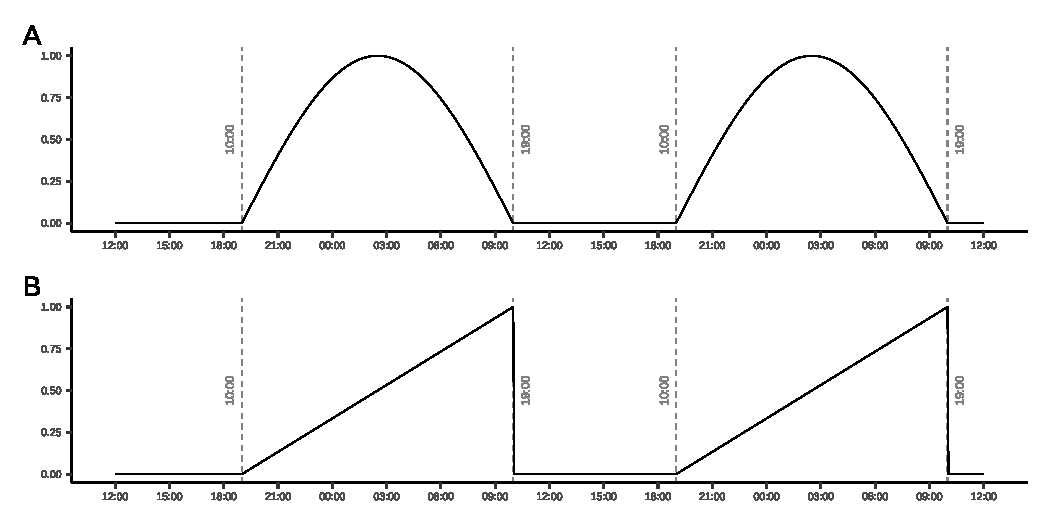
\includegraphics{visuals/sensor_independent.pdf}

}

\caption{\label{fig-sensor-independent}Sensor-independent features of
circadian rhythms across two consecutive nights. A) cosinus feature, B)
linear feature.}

\end{figure}

In addition to the engineered features, we chose to incorporate the
median-filtered raw predictions from the ZM device into our modeling
process. This decision stemmed from the understanding that children
typically undergo around five to eight sleep cycles per night, with
awakenings most likely occurring at the end of each
cycle\citep{galland_normal_2012}. Upon examining the raw ZM predictions,
we noted a significant overestimation in the number of awakenings per
night for the children in our study, exceeding what would be expected
based on typical sleep cycle patterns. In particular, many of these
brief awakenings could be considered as noise, which when present in the
data, can potentially hinder the learning process of machine learning
models by obscuring the underlying patterns that the models are trying
to learn, leading to less accurate predictions. Consequently, we elected
to train and evaluate our models using not only the raw ZM output, but
also versions that were subjected to 5-minute and 10-minute median
filters. This approach, by mitigating this noise, resulted in an
anticipated, more age-appropriate count of awakenings per night,
providing a more accurate depiction of children's sleep patterns (see
Figure~\ref{fig-zm-median}).

\begin{figure}[b]

{\centering 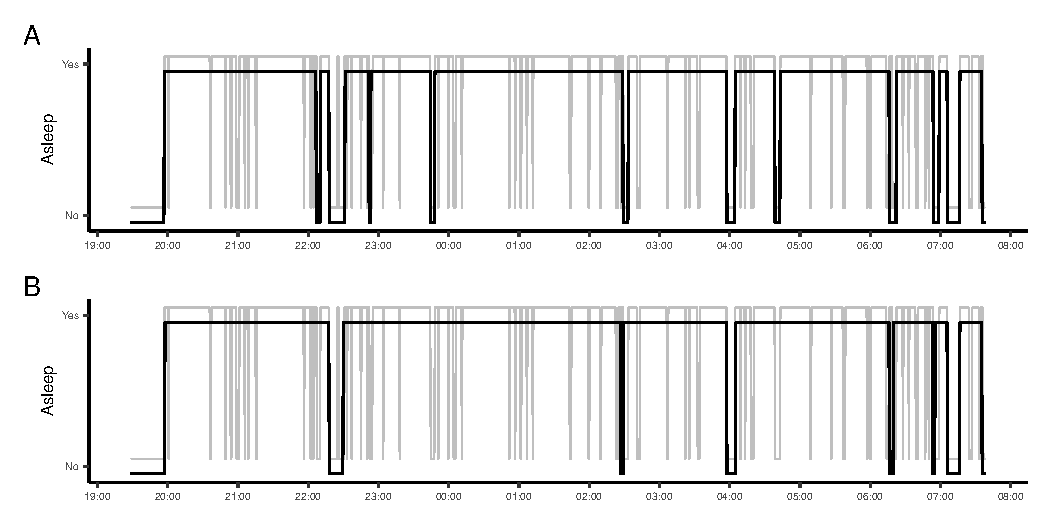
\includegraphics{visuals/zm_raw_vs_filtered.pdf}

}

\caption{\label{fig-zm-median}The difference in number of awakenings
between the raw ZM predictions vs.~5-minute, and 10-minute median
filtered predictions for a random night. Grey line is the raw
predictions, black line is the median filtered predictions. A: 5-minute
median filter on raw ZM predictions, B: 10-minute median filter on raw
ZM predictions.}

\end{figure}

\hypertarget{algorithms-training-and-validation}{%
\subsection{Algorithms, Training and
Validation}\label{algorithms-training-and-validation}}

In this study, we employed two distinct modeling strategies to analyze
sleep patterns from thigh-mounted accelerometer data. We used a
sequential strategy, comprising an ensemble of four pairs of models,
each pair featuring the same algorithm. This strategy aimed to make the
prediction task more manageable for the algorithms by breaking it down
into a sequence of two binary classifications: first predicting `in-bed'
time, then `sleep' time. Simultaneously, we also used a multiclass
approach utilizing a bidirectional Long Short-Term Memory
(biLSTM)\citep{hochreiter1997} neural network.

\hypertarget{models-in-sequence}{%
\subsubsection{Models in Sequence}\label{models-in-sequence}}

To predict in-bed time and sleep time accurately, we employed an
ensemble learning strategy based on sequential binary classification
models. This approach involved constructing a sequence of models using
multiple machine learning algorithms to improve predictive accuracy. The
process began with an initial model predicting in-bed time, followed by
a second model that utilized the output of the initial model to predict
sleep time. This sequential approach was applied across all four
algorithms detailed below, with each subsequent model leveraging the
outputs of the previous models for improved predictions.

\begin{enumerate}
\def\labelenumi{\arabic{enumi}.}
\item
  Logistic Regression (LREG): Logistic regression served as a simple and
  fast baseline model. However, due to its linear nature, it may
  struggle with capturing complex relationships and non-linear patterns
  present in the accelerometer data.
\item
  Decision Tree (TREE): Decision trees are capable of handling
  non-linear patterns and are easily interpretable. However, they are
  prone to overfitting, particularly when dealing with complex patterns
  that require simultaneous consideration of multiple features.
\item
  Single-layer Feed-forward Neural Network (SNN): Single-layer
  feed-forward neural networks can effectively capture non-linear
  relationships, even with their relatively simple structure. However,
  they tend to be more challenging to interpret compared to simpler
  models. Additionally, careful tuning of the network's architecture and
  training process is required to mitigate the risk of overfitting.
\item
  XGBoost (XGB): XGBoost is a powerful algorithm known for its ability
  to provide highly accurate predictions and handle complex, non-linear
  patterns in the data. It also incorporates built-in methods to prevent
  overfitting. However, training XGBoost models can be computationally
  intensive, and interpreting the predictions it generates can pose
  challenges.
\end{enumerate}

\hypertarget{multiclass-model}{%
\subsubsection{Multiclass Model}\label{multiclass-model}}

We also employed a biLSTM, a multiclass classifier, to predict three
distinct states: out-of-bed-awake, in-bed-awake, and in-bed-asleep. The
architecture of the biLSTM was set up with four layers, each equipped
with 128 hidden units. This configuration was intentionally chosen to
balance between model complexity and training efficiency: it provided
the depth necessary for learning intricate patterns while remaining
feasible for timely training. The bidirectional design of the LSTM
served to enhance data interpretation and mitigate overfitting by
doubling the hidden units at each time step. For input, we used tensors
shaped as sequences, with each sequence spanning 10 minutes and a step
size of one.This approach follows in the footsteps of previous studies
that utilized LSTM models for sleep detection. These studies showcased
the promising potential of LSTMs in capturing complex temporal patterns.
Particularly, the works of Sano et al. \citep{sano2019} and Chen et al.
\citep{chen2021} demonstrated the effectiveness of LSTM models in
improving sleep detection using accelerometer data, underscoring the
value of this modeling approach.

\hypertarget{model-training}{%
\subsubsection{Model Training}\label{model-training}}

For the models in sequence, we trained four pairs of classification
models. Each pair was designed to distinguish between in-bed/out-of-bed
and asleep/awake states, respectively. The dataset was randomly split
into a training set and a testing set, each containing approximately
50\% of the subjects. This division ensured that samples from the same
night were never simultaneously present in both sets. To optimize
hyperparameters, we performed a 10-fold Monte Carlo cross-validation on
a regular grid, comprising 20 different combinations of hyperparameters.
The F1 score served as the optimization metric. The best-performing set
of hyperparameters was then used to fit the models to the full training
dataset. This approach allowed us to maximize performance by leveraging
all available data. Moreover, after extracting the in-bed time from the
initial sequential models, the imbalance on the resulting dataset could
cause biases during model training, as models may favor predicting the
majority class. To rectify this, we employed the Synthetic Minority
Over-sampling Technique (SMOTE)\citep{chawla2002}. SMOTE generates new
samples by interpolating random samples with their nearest neighbors. We
utilized the themis R package\citep{themis} to implement SMOTE,
resulting in a balanced distribution of training samples across both
classes.

The biLSTM model was trained to differentiate between three states:
out-of-bed-awake, in-bed-awake, and in-bed-asleep. The data used for
training the biLSTM was randomly divided into training, validation, and
test sets, based on a 50/25/25 split. We ensured that data from the same
night was not present across different sets. The model was trained using
the Adam optimizer, selected for its computational efficiency and
adaptability of the learning rate during training. Given the multiclass
classification task with mutually exclusive classes, we employed the
cross-entropy loss function. To obtain a probability distribution over
the classes, the softmax activation function was applied at the output
layer. We evaluated the model's performance using the F1 score on both
the training and validation sets. We implemented early stopping with a
patience of 3 epochs, halting the training process if there was no
improvement in the validation loss over three consecutive epochs.

\hypertarget{model-validation}{%
\subsubsection{Model Validation}\label{model-validation}}

In our study, we utilized standard evaluation metrics to assess the
performance of each model on an epoch-to-epoch basis. These include
accuracy (\(accuracy = \frac{TP+TN}{TP+TN+FP+FN}\)), sensitivity
(\(sensitivity = \frac{TP}{TP+FN}\)), specificity
(\(specificity = \frac{TN}{TN+FP}\)), precision
(\(precision = \frac{TP}{TP+FP}\)), negative predictive value (NPV,
\(NPV = \frac{TN}{TN + FN}\)), and F1 score
(\(F_1 = 2 * \frac{precision * sensitivity}{precision + sensitivity}\)).

In the context of our sequential learning strategy, the initial models
were tasked with the binary classification of in-bed vs.~out-of-bed. For
this task, we assessed performance using the F1-score, accuracy,
sensitivity, specificity, and precision metrics. The second models in
our sequential learning strategy focused on the binary classification of
asleep vs.~awake. For these models, we considered the same metrics, in
addition to the negative predictive rate. The class imbalance in this
case led us to compute the F1 score as an unweighted macro-average.
Additionally, we evaluated the multiclass classifier, biLSTM, using the
same metrics. To do this, we considered the multiclass output as to
binary classifications, where the first was out-of-bed vs the rest and
the second binary classification as in-bed-awake vs in-bed-asleep. To
further illustrate model performance, we provide confusion matrices for
the full dataset, encompassing both in-bed and out-of-bed data. These
matrices report relative counts, column percentages (the proportion of
the true class accurately predicted), and row percentages (the
proportion of predictions correctly classified). We considered both the
in-bed/out-of-bed and awake/asleep scoring tasks as binary
classification problems, designating in-bed and asleep as the positive
labels and out-of-bed and awake as the negative labels in accordance
with previous research\citep{hjorth2012, kushida2001}.

To assess the performance of our models in deriving sleep quality
parameters, we utilized Bland-Altman plots and Pearson correlations. The
Bland-Altman method was employed specifically to determine the level of
agreement between two measurement techniques. Considering our dataset
contained multiple observations per subject, we integrated a bootstrap
procedure to address this extra source of variability. We calculated the
mean difference (bias) and defined the LOA as the mean difference plus
or minus 1.96 times the standard deviation of these differences. To
ensure our measurements were robust and accounted for intra-subject
variability, we estimated the 95\% confidence intervals for both the
bias and the LOA using a bias-corrected and accelerated bootstrap
method, utilizing 10,000 bootstrap replicates. The sleep quality
parameteres included are defined as follews in accordance with the ZM
definitions:

\begin{enumerate}
\def\labelenumi{\arabic{enumi}.}
\item
  Sleep Period Time (SPT) - This refers to the total duration of the
  sleep period, which is defined as the time from the start to the end
  of the ZM recording.
\item
  Total Sleep Time (TST) - This is the time spent asleep within the SPT.
\item
  Sleep Efficiency (SE) - This is the ratio between TST and SPT,
  representing the proportion of the sleep period that was actually
  spent asleep.
\item
  Latency Until Persistent Sleep (LPS) - This metric represents the time
  it takes to transition from wakefulness to sustained sleep. It is
  calculated as the time from the beginning of the ZM recording until
  the first period when 10 out of 12 minutes are scored as sleep.
\item
  Wake After Sleep Onset (WASO) - This refers to the time spent awake
  after initially falling asleep and before the final awakening. In our
  analysis, a period is counted as `awake' only if it consists of 3 or
  more contiguous 30-second epochs which is also how the ZM summarizes
  WASO.
\end{enumerate}

R version 4.3.0 (2023-04-21)\citep{R-lang} and the
Tidymodels\citep{tidymodels} and Tidyverse\citep{tidyverse} suite of
packages were used as the core tools for model development and analyses.
Python version 3.10.6\citep{10.5555/1593511} and
PyTorch\citep{NEURIPS2019_9015} were used to implement the biLSTM model.
All code used to perform the analysis and generate the figures in this
paper are available in
\href{https://github.com/esbenlykke/sleep_study}{this repository}.

\hypertarget{results}{%
\section{Results}\label{results}}

As reported in Table~\ref{tbl-zm_overview} the sleep quality parameters
derived from ZM predictions were modified by the implementation of
5-minute and 10-minute median filters. SPT were consistent across raw
and filtered datasets (mean: 9.2 ± 2.1 hours), corresponding to the
length of the ZM recording. TST and SE increased in the filtered data,
implying the filters categorize some wakefulness as sleep. Specifically,
TST increased from a raw mean of 7.7 ± 1.9 hours to 8.1 ± 2.0 hours
(5-minute filter) and 8.2 ± 2.1 hours (10-minute filter), while SE rose
from 82.6 ± 12.0\% to 86.4 ± 12.7\% and 87.5 ± 12.9\% respectively. LPS
also elevated, suggesting the filter smooths out brief awakenings at
sleep onset, leading to a prolonged time to persistent sleep. A
significant change was seen in WASO, which dropped from 39.0 ± 33.6
minutes in raw data to 30.6 ± 46.8 minutes and 22.3 ± 55.4 minutes in
the 5-minute and 10-minute filtered data, respectively. The number of
awakenings was also considerably reduced with the application of
filters. In the raw data, the average number of awakenings was 34.46 ±
11.33 per night, which reduced to 4.43 ± 3.26 and 1.95 ± 2.01 for the
5-minute and 10-minute filtered data sets respectively.

\hypertarget{tbl-zm_overview}{}
\begin{longtable}{lrrrrrr}
\caption{\label{tbl-zm_overview}Overview of characteristics of the ZM sleep quality summaries per night.
Values are represented as mean (SD). }\tabularnewline

\toprule
 & SPT (hrs) & TST (hrs) & SE (\%) & LPS (min) & WASO (min) & Awakenings (N) \\ 
\midrule
Raw ZM Predictions & 9.2 (2.1) & 7.7 (1.9) & 82.6 (12) & 34.5 (27.9) & 39 (33.6) & 34.5 (11.3) \\ 
5-Min Median & 9.2 (2.1) & 8.1 (2) & 86.4 (12.7) & 36.3 (39.8) & 30.6 (46.8) & 4.4 (3.3) \\ 
10-Min Median & 9.2 (2.1) & 8.2 (2.1) & 87.5 (12.9) & 38 (48.7) & 22.3 (55.4) & 1.9 (2) \\ 
\bottomrule
\end{longtable}

\hypertarget{performance-on-epoch-to-epoch-basis}{%
\subsection{Performance on Epoch-to-Epoch
Basis}\label{performance-on-epoch-to-epoch-basis}}

The epoch-to-epoch evaluation of predicting in-bed time is outlined in
Table~\ref{tbl-in_bed_performance}, and demonstrates practically
equivalent performance across all model types. The F1 score ranges from
94.4\% (Decision Tree) to 95.4\% (XGBoost), while accuracy ranges from
95.3\% (Decision Tree) to 96.1\% (XGBoost). Sensitivity, Precision, and
Specificity also demonstrate consistent results across the models. The
XGBoost model, despite recording the highest metrics with an F1 score of
95.4\% and accuracy of 96.1\%, outpaced the others only marginally.

\hypertarget{tbl-in_bed_performance}{}
\begin{longtable}{lrrrrr}
\caption{\label{tbl-in_bed_performance}In-bed performance metrics }\tabularnewline

\toprule
 & F1 Score (\%) & Accuracy (\%) & Sensitivity (\%) & Precision (\%) & Specificity (\%) \\ 
\midrule
Decision Tree & $94.4$ & $95.3$ & $93.1$ & $95.6$ & $96.9$ \\ 
Logistic Regression & $95.0$ & $95.7$ & $95.0$ & $94.9$ & $96.3$ \\ 
Feed-Forward Neural Net & $95.0$ & $95.8$ & $95.1$ & $95.0$ & $96.3$ \\ 
XGBoost & $95.4$ & $96.1$ & $95.8$ & $94.9$ & $96.2$ \\ 
biLSTM & $95.2$ & $95.3$ & $95.3$ & $95.1$ & $95.3$ \\ 
\bottomrule
\end{longtable}

Table~\ref{tbl-sleep_performance} details the performance of all
sequential model types on raw and median-filtered (5 and 10 minute) ZM
predictions for sleep/wake classification. For raw ZM predictions, the
F1 scores, which are unweighted macro averages, range from 65.6\%
(biLSTM) to 76.2\% (XGBoost). All models perform comparably, but the low
specificity values (62.5\% to 70.9\%) suggest difficulty in correctly
classifying awake epochs. Applying a 5-minute median filter improves the
performance metrics. The XGBoost model tops the charts with an F1 score
of 79.2\% and NPV of 74.0\%. However, specificity still remains low,
with values between 54.7\% (XGBoost) and 74.8\% (Logistic Regression)
across all models. With a 10-minute median filter, the metrics improve
further. The XGBoost model still leads with an F1 score of 80.9\% and an
NPV of 75.9\%. But, specificity remains low, ranging from 57.5\%
(Decision Tree) to 76.4\% (Logistic Regression) across all models.

\hypertarget{tbl-sleep_performance}{}
\begin{longtable}{lrrrrr}
\caption{\label{tbl-sleep_performance}Performance of the sleep/wake classification of the sequential models. }\tabularnewline

\toprule
 & F1 Score (\%) & Precision (\%) & NPV (\%) & Sensitivity (\%) & Specificity (\%) \\ 
\midrule
\multicolumn{6}{l}{Raw ZM Predictions} \\ 
\midrule
Decision Tree & $72.9$ & $93.2$ & $48.4$ & $86.3$ & $67.1$ \\ 
Logistic Regression & $71.0$ & $93.7$ & $43.9$ & $82.7$ & $70.9$ \\ 
Neural Network & $71.8$ & $93.8$ & $45.1$ & $83.6$ & $70.8$ \\ 
XGBoost & $76.2$ & $92.8$ & $58.0$ & $91.3$ & $62.8$ \\ 
biLSTM & $65.6$ & $80.6$ & $80.6$ & $62.5$ & $62.5$ \\ 
\midrule
\multicolumn{6}{l}{5-Min Median} \\ 
\midrule
Decision Tree & $75.5$ & $94.2$ & $55.5$ & $93.4$ & $59.0$ \\ 
Logistic Regression & $68.3$ & $95.8$ & $36.0$ & $81.4$ & $74.8$ \\ 
Neural Network & $71.7$ & $95.8$ & $41.6$ & $85.6$ & $73.1$ \\ 
XGBoost & $79.2$ & $93.9$ & $74.0$ & $97.3$ & $54.7$ \\ 
biLSTM & $70.3$ & $84.6$ & $84.6$ & $66.2$ & $66.2$ \\ 
\midrule
\multicolumn{6}{l}{10-Min Median} \\ 
\midrule
Decision Tree & $76.3$ & $94.7$ & $58.1$ & $94.9$ & $57.5$ \\ 
Logistic Regression & $68.0$ & $96.5$ & $34.3$ & $81.9$ & $76.4$ \\ 
Neural Network & $71.0$ & $96.1$ & $39.5$ & $86.5$ & $71.4$ \\ 
XGBoost & $80.9$ & $94.9$ & $75.8$ & $97.7$ & $57.6$ \\ 
biLSTM & $70.9$ & $75.1$ & $75.1$ & $68.5$ & $68.5$ \\ 
\bottomrule
\end{longtable}

A complete set of confusion matrices generated from data both containing
the out-of-bed and in-bed time are presented in
Figure~\ref{fig-conf_mat}. The figure shows favorable epoch-to-epoch
performance across across all sequential models, however, it is evident
that the biLSTM is less successful in classifying the in-bed-awake class
which cannot be deduced from the confusion matrices from the sequential
models.

\begin{figure}[b]

{\centering \includegraphics{visuals/all_conf_mats.pdf}

}

\caption{\label{fig-conf_mat}Confusion matrices for binary sleep
prediction. The middle of each tile is the normalized count (overall
percentage) and, beneath it, the count. The bottom number is the column
percentage (target). At the right side of each tile is the row
percentage (prediction). i) decision tree, ii) logistic regression, iii)
feed-forward neural net, iv) XGBoost, and v) biLSTM.}

\end{figure}

\hypertarget{evaluation-of-sleep-quality-parameters}{%
\subsection{Evaluation of Sleep Quality
Parameters}\label{evaluation-of-sleep-quality-parameters}}

Table~\ref{tbl-ba_cor} presents a comparative analysis of the included
models used to predict various sleep quality parameters (SPT, TST, SE,
LPS, WASO) using the 5-minute median filtered ZM predictions. To see the
full table including models developed from raw ZM predictions and
10-minute median filtered ZM predictions, see \textbf{{[}SUPP. MAT.{]}}.
In terms of bias, the decision tree model consistently underestimated
SPT, TST, and SE, and overestimated LPS and WASO in comparison to ZM.
The logistic regression model had similar trends, with more pronounced
underestimation in TST and overestimation in LPS. The eed-forward neural
network also exhibited similar bias as the decision tree and the
logistic regression models, but with a higher overestimation in WASO. On
the other hand, the XGBoost model showed least bias among all,
especially in its 5-minute median predictions. Considering LOA, the
decision tree had higher variability across different sleep quality
parameters and filtering techniques, particularly for LPS and WASO,
which indicates lower agreement with ZM. Other models had comparable LOA
but with notable exceptions. For example, TST LOA for the logistic
regression model was particularly wide in the 5-minute median
predictions. Correlation-wise, the pearson coefficient, revealed that
the XGBoost model consistently had the highest correlation with ZM
across all sleep qualityparameters and filtering methods Notably, the
XGBoost's 5-minute median predictions showed the strongest correlation
(0.66) for TST among all models and filtering techniques.

\hypertarget{tbl-ba_cor}{}
\begin{longtable}{lrrrr}
\caption{\label{tbl-ba_cor}Summary of Bias, Limits of Agreement, and Pearson Correlation for
various Sleep Parameter Predictions (SPT, TST, SE, LPS, WASO) using
different Machine Learning Models (Decision Tree, Logistic Regression,
Feed-Forward Neural Net, XGBoost) with Raw ZM Predictions, 5-Min and
10-Min Median as predictors. Each value is provided with its 95\%
Confidence Interval (CI). }\tabularnewline

\toprule
 & Bias (95\% CI) & LOA (95\% CI) & LOA (95\% CI) & Pearson, \emph{r} (95\% CI) \\ 
\midrule
\multicolumn{5}{l}{5-Min Median - Decision Tree} \\ 
\midrule
SPT (min) & -21.6 (-25.6;-17.6) & -117.5 (-125.6;-110.7) & 74.2 (63.9;85.9) & 0.54 (0.48;0.6) \\ 
TST (min) & -50.5 (-55.2;-46) & -161.4 (-175.8;-151.3) & 60.4 (51.5;71.7) & 0.48 (0.42;0.54) \\ 
SE (\%) & -5.5 (-6.3;-4.7) & -23.9 (-26.4;-22.2) & 12.9 (11.6;14.6) & 0.22 (0.14;0.29) \\ 
LPS (min) & 24.6 (19.7;29.1) & -88.8 (-115;-77.3) & 138 (126.2;156.7) & 0.06 (-0.02;0.14) \\ 
WASO (min) & 9.9 (6.5;14) & -79.4 (-109;-63.1) & 99.2 (80;136.1) & 0.15 (0.07;0.22) \\ 
\midrule
\multicolumn{5}{l}{5-Min Median - Logistic Regression} \\ 
\midrule
SPT (min) & -3.7 (-8;1) & -112.2 (-120.9;-105.2) & 104.8 (94;117.4) & 0.38 (0.3;0.44) \\ 
TST (min) & -139.7 (-146.9;-133) & -305.6 (-323.6;-291.8) & 26.2 (16.1;38.6) & 0.09 (0.01;0.17) \\ 
SE (\%) & -23.2 (-24.3;-22.2) & -48.1 (-50.9;-46.1) & 1.7 (0.1;3.8) & 0.13 (0.05;0.21) \\ 
LPS (min) & 58.1 (53.4;62.6) & -52.3 (-75;-40.1) & 168.6 (155.9;187.7) & 0.05 (-0.03;0.13) \\ 
WASO (min) & 45.4 (41.7;49.7) & -50.7 (-74.4;-38.4) & 141.5 (126.8;173) & 0.19 (0.11;0.27) \\ 
\midrule
\multicolumn{5}{l}{5-Min Median - Feed-Forward Neural Net} \\ 
\midrule
SPT (min) & -3.9 (-8.1;0.9) & -112.7 (-122;-105.2) & 104.9 (94.1;118.4) & 0.38 (0.3;0.44) \\ 
TST (min) & -126.5 (-132.8;-120.3) & -276.8 (-291.3;-264.7) & 23.9 (14.8;33.9) & 0.25 (0.17;0.32) \\ 
SE (\%) & -20.9 (-21.9;-19.9) & -44.3 (-46.3;-42.5) & 2.5 (1.1;4) & 0.21 (0.13;0.29) \\ 
LPS (min) & 35.3 (30.7;39.8) & -75.8 (-102.3;-63.4) & 146.5 (134.4;166.9) & 0.07 (-0.01;0.15) \\ 
WASO (min) & 45 (41.2;49.2) & -51.8 (-76.4;-39.1) & 141.7 (125.8;174.1) & 0.21 (0.14;0.29) \\ 
\midrule
\multicolumn{5}{l}{5-Min Median - XGboost} \\ 
\midrule
SPT (min) & 0.2 (-3.7;4.5) & -97.4 (-106.2;-90.3) & 97.8 (86.6;111) & 0.56 (0.5;0.61) \\ 
TST (min) & -7 (-10.8;-3.3) & -95.5 (-105.2;-88) & 81.4 (72.4;92.5) & 0.66 (0.61;0.7) \\ 
SE (\%) & -1.1 (-1.7;-0.5) & -15.6 (-17;-14.4) & 13.3 (12.2;14.7) & 0.44 (0.38;0.51) \\ 
LPS (min) & 28.5 (23.9;32.6) & -76.4 (-104.2;-63.3) & 133.4 (120.4;154.2) & 0.12 (0.04;0.2) \\ 
WASO (min) & -0.9 (-3.9;3) & -83.4 (-113.1;-66) & 81.7 (62;119.6) & 0.26 (0.18;0.33) \\ 
\midrule
\multicolumn{5}{l}{5-Min Median - biLSTM} \\ 
\midrule
SPT (min) & -36.1 (-41.7;-30) & -136.1 (-146.3;-126.9) & 64 (51.1;78.6) & 0.54 (0.45;0.62) \\ 
TST (min) & 12.8 (7.4;18.3) & -80.1 (-89.8;-72.3) & 105.8 (94.3;118.8) & 0.63 (0.55;0.69) \\ 
SE (\%) & 8 (7.2;8.8) & -5.1 (-6.8;-3.8) & 21.1 (19.5;23.1) & 0.16 (0.04;0.27) \\ 
LPS (min) & -15.7 (-25.9;-7.5) & -169 (-230.7;-127.9) & 137.6 (101.1;184.9) & 0.09 (-0.02;0.2) \\ 
WASO (min) & -3 (-9.9;7.7) & -144.1 (-197.2;-107.2) & 138.1 (90.8;211.4) & 0.02 (-0.1;0.13) \\ 
\bottomrule
\end{longtable}

Figure~\ref{fig-xgb_ba_cor} shows the agreement between the XGBoost
model, trained on 5-minute median filtered ZM predictions, and the
5-minute median-smoothed ZM-derived sleep quality parameters. The
Bland-Altman plot for the SPT reveals a significant level of agreement
with the ZM, as evidenced by a positive correlation. However, the
presence of extreme outliers widens the limits of agreement (LOA). The
scatterplot for SPT also demonstrates a positive trend, indicating a
moderate linear correlation between the XGBoost model and the ZM-derived
sleep quality parameters.In terms of TST, perfect agreement is not
observed for a substantial number of nights, but there is a positive
correlation between the XGBoost model and ZM-derived sleep quality
parameters. The bias and LOA for TST are comparable to those observed
for SPT, indicating a consistent level of agreement between the two
methods. The scatterplot for TST also shows a slightly higher
correlation, primarily driven by the absence of extreme
outliers.Furthermore, the remaining three sleep quality parameters, SE,
LPS, and WASO, exhibit heteroscedasticity in contrast to SPT and TST.
This outcome is expected as achieving 100\% sleep efficiency is
relatively rare, resulting in less disagreement between the methods as
values approach the upper limit. However, as sleep efficiency decreases,
the potential for discrepancies and differing interpretations between
the methods increases, leading to greater heteroscedasticity. A moderate
linear correlation is observed between the XGBoost model and ZM-derived
sleep quality parameters for SE, indicating a positive relationship.
However, a poor correlation is observed for LPS and WASO, suggesting
less agreement between the two methods for these parameters. Similar
plots for all models are available in the supplementary materials.

\begin{figure}[b]

{\centering \includegraphics{visuals/median_5_xgboost_ba_cor.pdf}

}

\caption{\label{fig-xgb_ba_cor}Comparison of sleep quality parameters
derived from the XGBoost model trained on the 5-minute smoothed ZM
predictions. The left column displays Bland-Altman plots. Dashed lines
represent the bias (the average difference between the two measurements)
and LOA, with the 95\% confidence intervals represented as the grayed
areas. The right column displays scatter plots of XGBoost-derived vs
ZM-derived sleep quality parameters. The dashed line represents the
identity line, while the full-drawn line represents the best linear fit.
Pearson's correlations are annotated in the upper left corner.}

\end{figure}

\hypertarget{discussion}{%
\section{Discussion}\label{discussion}}

In an effort to mature the methods for estimating sleep from thigh-worn
accelerometers, we evaluated various models for predicting in-bed and
sleep time and their derived sleep quality parameters. Furthermore, we
trained and evaluated the models using raw and median-filtered gold
standard predictions from the ZM. In general, all sequential models
performed well at predicting in-bed time. More challenging was it to
distinguish wake from sleep on the extracted in-bed time, however, the
performance of the sequential models were enhanced by the application of
median filters. Moreover, even though the multiclass biLSTM showed good
performance across F1 score, precision and NPV, the derived sleep
quality parameters were not on par with the XGBoost model which
demonstrated the highest performance metrics across all evaluations,
including epoch-to-epoch prediction and sleep quality parameter
derivatives. Despite this, all sequential models showed low specificity
values, indicating difficulty in correctly classifying awake epochs
during time in bed. The application of 5-minute and 10-minute median
filters improved the performance metrics of all models, with the XGBoost
model consistently leading. The median filters increased total sleep
time and sleep efficiency, while reducing wake after sleep onset and the
number of awakenings. The XGBoost model also showed the least bias and
highest correlation with ZM across sleep quality parameters.

Limited research exists regarding the epoch-to-epoch effectiveness of
classifying in-bed time based on data from thigh-worn accelerometers.
Nevertheless, Carlson and colleagues provided compelling insights. They
demonstrated that a third-party algorithm, ``ProcessingPal,'' and a
proprietary one, ``CREA,'' achieved accuracies of 91\% and 86\%
respectively. These algorithms, evaluated against self-reported
measures\citep{carlson2021}, produced F1 scores as high as 95\% and
96\%. These figures are consistent with the performance of our
sequential models, which also achieved F1 scores and accuracy scores
exceeding 95\% in identifying in-bed time. In our study, in-bed time is
equated with SPT. All models, with the exception of XGBoost,
underestimated SPT. The biLSTM model showed the greatest
underestimation, with a bias of -36 minutes, reflecting trends observed
in previous research. Winkler et al. developed an algorithm that,
despite a strong correlation (Pearson correlation coefficient = .67)
between their algorithmic results and diary-recorded waking times,
overestimated waking wear time by more than 30 minutes, resulting in an
underestimation of in-bed time\citep{winkler2016}. This trend was
further confirmed when Inan-Eroglu et al.~examined Winkler et al.'s
algorithm, revealing a underestimation of 9.8 minutes in bed time
compared to self-reported measures\citep{inan-eroglu2021}. In contrast,
a study by van der Berg et al. reported a slight underestimation of
in-bed time. They employed a unique approach with their algorithm, which
relied on quantifying the number and duration of sedentary periods to
determine time in bed, and active periods (standing or stepping) to
identify wake times\citep{vanderberg2016}. Finally. it is important to
note that high predictive performance in determining in-bed time does
not necessarily translate to accurate predictions of broader sleep
quality parameters. The crucial task of detecting awake periods during
in-bed time, a key factor in assessing sleep quality, may not be
effectively captured by in-bed time predictions alone. Indeed,
underestimating in-bed time could result in overestimating waking time
during in-bed time. Furthermore, the distinction between actual sleep
and time spent in bed, often overlooked but vital in sleep research, is
critical for a comprehensive understanding of sleep quality.

To the best of our knowledge, Johansson and
colleagues\citep{johansson_development_2023} are the only researchers
who have reported epoch-to-epoch performance metrics for sleep scoring
using thigh-worn accelerometers, beyond just ``waking time'' and
``in-bed time.'' They achieved a mean sensitivity of 0.84, specificity
of 0.55, and accuracy of 0.80, using a single-night evaluation dataset
of 71 subjects. Despite our models achieving a sensitivity above 97\%,
they, like Johansson et al.'s algorithm, struggled with detecting in-bed
awake epochs. This is reflected in the low specificity scores, ranging
from 54.7\% to 76.4\%, reported in our study. The challenge of low
specificity is not unique to methods using data collected from
thigh-worn devices. Conley et al.'s meta-analysis\citep{conley2019}
reported similar findings when estimating sleep using wrist-worn
accelerometers among healthy adults, with a mean sensitivity, accuracy,
and specificity of 0.89, 0.88, and 0.53, respectively. Furthermore,
Patterson and colleagues\citep{patterson_40_2023} recently summarized
the performance of various heuristic algorithms, machine learning, and
deep learning models used to predict sleep. They found the mean
sensitivity and specificity to be 93\% (SD = 2.8) and 60\% (SD = 11.1)
respectively. These findings underscore the challenge of automating the
detection of in-bed awake periods. Interestingly, despite low
specificity values for most of our models and configurations, we
observed an overestimation of LPS and WASO, contrasting with most
previous research\citep{conley2019, palotti2019}. This overestimation of
wake epochs is evident from the low NPV scores, indicating that only a
small proportion of the wake predictions are actually correct. This
discrepancy may be driven by the SMOTE process used to balance the
dataset. If the synthetic ``wake'' samples created by SMOTE are not
representative of the true ``wake'' data, the models might learn to
incorrectly classify certain ``sleep'' epochs as ``wake''. This could
lead to an overestimation of LPS and WASO, as the models are incorrectly
identifying more periods of wakefulness during the sleep period.

The use of the SMOTE technique likely improved the performance of our
models by addressing the class imbalance in our data. However, this
technique also introduced synthetic''wake'' samples that may not be
fully representative of true wake data. This could potentially lead some
models to overestimate the wake class. Interestingly, the biLSTM model,
which was not trained on SMOTE-processed data, was the only one to
overestimate TST and SE. On the other hand, the XGBoost model, which was
trained on data subjected to the SMOTE process, was able to handle the
synthetic ``wake'' samples better than the other models, and it did not
overestimate TST to the same degree. The Bland-Altman statistics for the
XGBoost model trained on the 5-minute median filtered ZM predictions
showed a mean difference of -7 minutes for TST and -1.1\% for SE, with
limits of agreement ranging from -95.5 to 81.4 minutes and from -15.6\%
to 13.3\% respectively. This suggests that the XGBoost model was able to
maintain a balance between sensitivity and specificity, and it was not
overly influenced by the synthetic ``wake'' samples. The XGBoost model's
success with the SMOTE dataset may be due to its ability to handle
non-representative synthetic samples. XGBoost's gradient boosting
mechanism allows it to iteratively learn from the errors of previous
models, which can help it to better distinguish between true wake data
and synthetic wake samples created by SMOTE. This iterative learning
process could make XGBoost more robust to the inaccuracies introduced by
the synthetic samples, leading to better overall performance.

In our evaluation of sleep quality parameters, we found that Latency to
Persistent Sleep (LPS) had the largest mean error relative to absolute
time allocated to LPS. This suggests that the initial epochs of Sleep
Period Time (SPT) are particularly challenging to classify correctly.
This is also supported by the poor Pearson correlations between LPS
derived from model predictions and the ZM. The XGBoost model, which was
the best performer among all models, overestimated LPS by an average of
26.4 minutes for models trained on raw ZM predictions, 28.5 minutes for
models trained on 5-minute filtered ZM predictions, and 34.5 minutes for
models trained on 10-minute filtered ZM predictions. This level of
discrepancy is comparable to the mean error of sleep latency of 23
minutes reported by Johansson et al.\citep{johansson_development_2023}.
Johansson et al.~suggest that the discrepancy with the gold standard is
likely due to the multifaceted nature of the sleep state, which is a
complex physiological process. Short awakenings or sleep episodes may
not necessarily correspond to noticeable changes in thigh movement,
making them difficult to detect and accurately classify. These results
align with several methods for wrist-worn devices reviewed by Conley and
colleagues\citep{conley2019}. They reported correlations between
accelerometer and PSG sleep onset latency (equivalent to LPS) from 10
studies with a mean correlation of 0.2 (ranging from -0.69 to 0.69),
indicating the inherent difficulty in estimating this parameter using
accelerometry alone.

In this study, we used the ZM as the reference method, rather than PSG,
which is considered the gold standard for sleep measurement. This choice
may contribute to discrepancies between our models and the ZM, as
without a true gold standard, it's difficult to determine the source of
disagreement. However, we believe that the use of ZM, which allows for
multiple consecutive nights of recording, is valuable. This approach
captures intra-individual variances in sleep, which is impractical with
PSG. It also enabled us to include more nights in our study typically
compared to those relying on PSG. For instance, the widely used
Newcastle dataset\citep{hees2015} only contains data from 28
participants. However, upon examining the ZM outputs, we found that the
raw predictions were not optimal for developing machine learning models
due to a seemingly low signal-to-noise ratio (see
Figure~\ref{fig-zm-median}). The ZM itself mitigates this issue by
applying certain filtering processes when generating sleep quality
parameters. For example, epochs contributing to WASO must be in
contiguous epochs of 3, and sleep only counts towards sleep quality
parameters if 10 out of 12 minutes are scored as sleep. To improve the
prospect of our machine learning algorithms, we applied median filters
to the ZM raw predictions. This did in fact alter the derived sleep
quality parameters. Notably, the mean WASO decreased from 39 minutes in
the raw predictions to 30.6 minutes in the 5-minute median filtered
predictions, and further decreased to 22.3 minutes in the 10-minute
filtered predictions. The application of 5-minute and 10-minute median
filters also led to increases in TST, SE, and LPS. This suggests that
the filters may categorize some instances of wakefulness as sleep and
smooth out brief awakenings. Despite these changes, the overall sleep
quality profile derived from the median-filtered predictions is still
comparable to that from the raw predictions, justifying our approach.

Our study's XGBoost model demonstrated relatively narrower limits of
agreements (LOAs) for TST, SE, and WASO, with ranges of -95.5 to 81.4
min, -15.6 to 13.3\%, and -83.4 to 81.7 min, respectively when compared
with other models such as the Van Hees algorithm\citep{hees2015}, Oakley
rsc (rescored)\citep{palotti2019}, and LSTM-50\citep{palotti2019}
evaluated in the Patterson et al.~study\citep{patterson_40_2023}.
Furthermore, comparing the LOAs between our XGBoost model and the
algorithm developed for thigh-worn devices by Johansson et
al.~study\citep{johansson2022}, our XGBoost model showed narrower LOAs
for TST , SE, LPS , and WASO, but not SPT. Generally, all methods, both
from this study and from the reviewed literature, exibit wide LOAs
sugesting that there is high variability in the derevide sleep quality
parameters. These findings imply that the current methods, are only
reasonbly reliable for assessing sleep quality parameters at a group
level. However, caution should be exercised when applying the models and
methods to individual-level sleep assessments. Therefore, further
improvements and refinements are needed to enhance the precision and
reliability of these models for individual sleep assessments.

Typically, sleep detection methods are applied in two contexts: either
to night recordings or to 24-hour recordings. In night recordings, it is
often possible to derive sleep quality parameters like SE and LPS
because the SPT is already known. This knowledge usually comes either
from sleep diaries\citep{girschik2012} or from the length of the
recording itself. On the other hand, when sleep detection methods are
applied to 24-hour recordings, most methods do not have the ability to
infer the SPT. Consequently, these methods are unable to generate
certain sleep quality parameters that rely on the
SPT\citep{doherty2017, anderson2014}.

Strengths and limitations It is not always clear the methods for
detecting sleep from accelerometer data is

It is unclear whether Johansson et al.\citep{johansson_development_2023}
provide a method for detecting the in-bed time which hinders its
applicability for researchers that want to \ldots{}

external validation dataset/generalization

expand the feature set (Palotti)

In conclusion, our study has advanced the methods for estimating sleep
from thigh-worn accelerometers by evaluating various models for
predicting in-bed and sleep time. Our results indicate that all
sequential models and the multiclass model performed well at predicting
in-bed time. However, all models showed difficulty in correctly
classifying awake epochs during time in bed, highlighting the challenge
of automating the detection of in-bed awake periods. The application of
median filters improved the performance metrics of all models,
suggesting that this approach may be beneficial in future studies.
Despite these promising results, our findings also underscore the need
for caution when applying these models to individual-level sleep
assessments due to the high variability in derived sleep quality
parameters. Future research should focus on refining these models to
enhance their precision and reliability for individual sleep
assessments.

Our open-source algorithm and the inferred sleep parameters will open
the door to future studies on sleep and sleep architecture using
large-scale accelerometer databases.

\newpage


\renewcommand\refname{References}
  \bibliography{bibliography.bib}


\end{document}
